\documentclass{frontiersSCNS}
\usepackage{url,hyperref,lineno,microtype,subcaption}
\usepackage[onehalfspacing]{setspace}
\usepackage{float}


\linenumbers

\usepackage[utf8]{inputenc}
\floatplacement{figure}{H}

\def\keyFont{\fontsize{8}{11}\helveticabold }
\def\firstAuthorLast{Villaseñor-Derbez {et~al.}}
\def\Authors{Juan Carlos Villaseñor-Derbez\(^{1,*}\), Eréndira
Aceves-Bueno\(^{1,*}\), Stuart Fulton\(^{2}\)}
% Affiliations should be keyed to the author's name with superscript numbers and be listed as follows: Laboratory, Institute, Department, Organization, City, State abbreviation (USA, Canada, Australia), and Country (without detailed address information such as city zip codes or street names).
% If one of the authors has a change of address, list the new address below the correspondence details using a superscript symbol and use the same symbol to indicate the author in the author list.
\def\Address{\(^{1}\)Bren School of Environmental Science and Management, University
of California, Santa Barbara, Santa Barbara, CA,
USA\newline \(^{2}\)Comunidad y Biodiversidad A.C., Guaymas, Mexico}
% The Corresponding Author should be marked with an asterisk
% Provide the exact contact address (this time including street name and city zip code) and email of the corresponding author
\def\corrAuthor{Juan Carlos Villaseñor-Derbez, Bren Hall, University of California,
Santa Barbara, Santa Barbara, CA, 93106}

\def\corrEmail{\href{mailto:jvillasenor@bren.ucsb.edu}{\nolinkurl{jvillasenor@bren.ucsb.edu}}}

\usepackage{amsthm}
\newtheorem{theorem}{Theorem}[section]
\newtheorem{lemma}{Lemma}[section]
\theoremstyle{definition}
\newtheorem{definition}{Definition}[section]
\newtheorem{corollary}{Corollary}[section]
\newtheorem{proposition}{Proposition}[section]
\theoremstyle{definition}
\newtheorem{example}{Example}[section]
\theoremstyle{definition}
\newtheorem{exercise}{Exercise}[section]
\theoremstyle{remark}
\newtheorem*{remark}{Remark}
\newtheorem*{solution}{Solution}
\begin{document}
\onecolumn
\firstpage{1}

\title[Mexican marine reserves]{Cool title here} 

\author[\firstAuthorLast ]{\Authors} %This field will be automatically populated
\address{} %This field will be automatically populated
\correspondance{} %This field will be automatically populated

\extraAuth{}

\maketitle



\begin{abstract}

Abstract here




\medskip
\tiny
 \keyFont{ \section{Keywords:} Marine Reserves, Marine Conservation, Small Scale Fisheries, Citizen
Science, Mexico, Social--Ecological Systems}



\end{abstract}


\section{Introduction}\label{introduction}

Marine ecosystems around the world sustain significant impacts due to
overfishing and unsustainable fishing practices
\citep{halpern_2008-dK,worm_2006-IB,pauly_2005-qV}. A common approach to
manage the spatial distribution of fishing effort and recover stocks is
through the implementation of marine reserves (\emph{i.e.} areas where
all fishing activities are off--limits; MRs)
\citep{afflerbach_2014-HP,krueck_2017-J1,sala_2017-69}.

Marine reserve science has largely focused on understanding the
ecological effects of these areas, which include increased biomass,
richness, and densities of organisms within the protected regions
\citep{lester_2009-Ks,giakoumi_2017-V2,sala_2017-69}, climate change
mitigation \citep{roberts_2017-J9}, and protection from environmental
variability \citep{micheli_2012-EU}. However, there is considerably less
literature focusing on the relationship between socioeconomic and
governance structures and their relationship to ecological
effectriveness \citep{halpern_2013,lpezangarita_2014,mascia_2017-m_} or
benefits to fisheries \citep{krueck_2017-J1}; evaluations of marine
reserves rarely provide a hollistic view of the social-ecological system
\citep{lpezangarita_2014}. Here, we combine causal inference techniques
\citep{depalma_2018} and the social-ecological systems framework
\citep{ostrom_2009-hg} to provide a comprehensive ecological and
socioeconomic evaluation of four community-based marine reserves in
three coastal communities in Mexico.

Marine Reserves in Mexico have been commonly implemented as ``core
zones'' within Biosphere Reserves (BRs) that are administered by the
National Commision of Protected Areas (\emph{Comisión Nacional de Áreas
Marinas Protegidas}, CONANP). While CONANP has made efforts to have a
participatory process, the implementation of these zones is still
characterized by top--down approaches. This motivated Civil Society
Organizations (CSOs) to work with coastal communities to implement
community--based marine reserves \citep{uribe_2010-u2}, which are
usually established within a Territorial Use Rights for Fisheries
(TURFs); thus making them TURF--reserves \citep{afflerbach_2014-HP}.
This bottom--up approach allows fishers to disign their own reserves,
which increases compliance and self--enforcement
\citep{gelcich_2015-Gw,espinosaromero_2014-PY,beger_2004-Y8}. However,
these reserves still lack legal recognition, making them vulnerable to
poaching. In 2014, a new norm \citep{nom} allowed fishers to request the
legal recognition of a community--based reserve under the name of
``Fishing Refugia'' (\emph{Zona de Refugio Pesquero}, FR). This new norm
thus combines bottom--up approaches to design marine reserves, along
with a legal recognition of the management intervention. Since then,
\emph{39} FR have been implemented along the Pacific, Gulfof
Caloifornia, and Mexican Caribbean coastlines, but no formal evaluation
of their effectiveness has taken place.

While there are ecological factors defining the success of a MR
(\emph{i.e.} habitat representation, initial state of protection,
connectivity to other protected areas), their effectivness also depends
on the socioeconomic and governance settings under which they are
implemented. Literature shows that many non-ecological characteristics
can play an equally important role in the effectivenes of MRs. For
example, age of a reserve (\emph{i.e.} time since its implementation),
size, and habitat contained were key to the effectiveness of MRs in
Palau \citep{friedlander_2017-oI}. In the Mediterranean,
\citet{difranco_2016-Xw} identify that surveilance and enfocrement,
presence of a management plan, and involvement of fishers in management
and decision--making along with promotion of sustainable fishing
practices were the key fators that increased stock health and income to
fishers. At a global level, \citet{edgar_2014-UO} indicate that
enforcement, age, size, and isolation were important factors determining
effectiveness of the reserves.

The objective of this work is twofold: i) Provide the first evaluation
of community--based marine reserves in Mexico, and ii) provide a
comprehensive evaluation of the social--ecological system to identify
how sociocoenomic and governance characteristics relate to ecological
effectiveness. With the purpose of providing a hollistic evaluation, we
combine ecological, socioeconomic, and governance indicators. We use
causal inference techniques to provide a measurement of the effect of
the management intervention, and combine it with the social--ecological
systems framework \citep{ostrom_2009-hg}.

\section{Materials and Methods}\label{materials-and-methods}

\subsection{Study area}\label{study-area}

We focus our evaluation in three coastal communities from the Pacific
coast of Baja California (n = 1) and the Mesoamerican Reef System (n =
2; Fig \ref{fig:map}). Isla Natividad (IN) lies west of the Baja
California Peninsula (Fig \ref{fig:map}B), where kelp forests
(\emph{Macrocystis pyrifera}) and rocky reefs are the predominant
habitats. The island is home to a fishing cooperative (\emph{Sociedad
Cooperative de Producción Pesquera Buzos y Pescadores de la Baja
California SCL}), that holds a TURF for spiny lobster (\emph{Panulirus
interruptus}). However, other resources like finfish (yellowtail jack,
\emph{Seriola lalandi}), sea cucumber (\emph{Parastichopus
parvimensis}), red sea urchin (\emph{Mesocentrotus franciscanus}), snail
(\emph{Megastraea turbanica} y \emph{M. undosa}), and abalone
(\emph{Haliotis spp}, until 2010) are also important sources of income.
In 2006, the community decided to implement two community--based marine
reserves within their fishing grounds, seeking to recover depleted
stocks of invertebrate species (mainly lobster and abalone). Until
today, these reserves are yet to be legally recognized as Fishing
Refugia.

The other two communities are Maria Elena (ME; Fig \ref{fig:map}C) and
Punta Herrero (PH; Fig \ref{fig:map}D) in the Yucatan Peninsula, where
coral reefs and mangroves are the representative coastal ecosystems. ME
is a fishing camp --visited intermitently during the fishing season--
belonging to the Cozumel fishing cooperative. PH is home to the ``José
María Azcorra'' fishing cooperative. The main source of income to both
communities is the caribbean spinly lobster fishery (\emph{Panulirus
argus}), which is carried out within their respective TURFs. These
communities also target finfish in the off season, mainly snappers
(Lutjanidae) and groupers (Serranidae). ME established eight marine
reserves in 2012, and PH established four marine reserves in 2013. All
these reserves are legally recognized as Fishing Refugia.

\begin{figure}
\centering
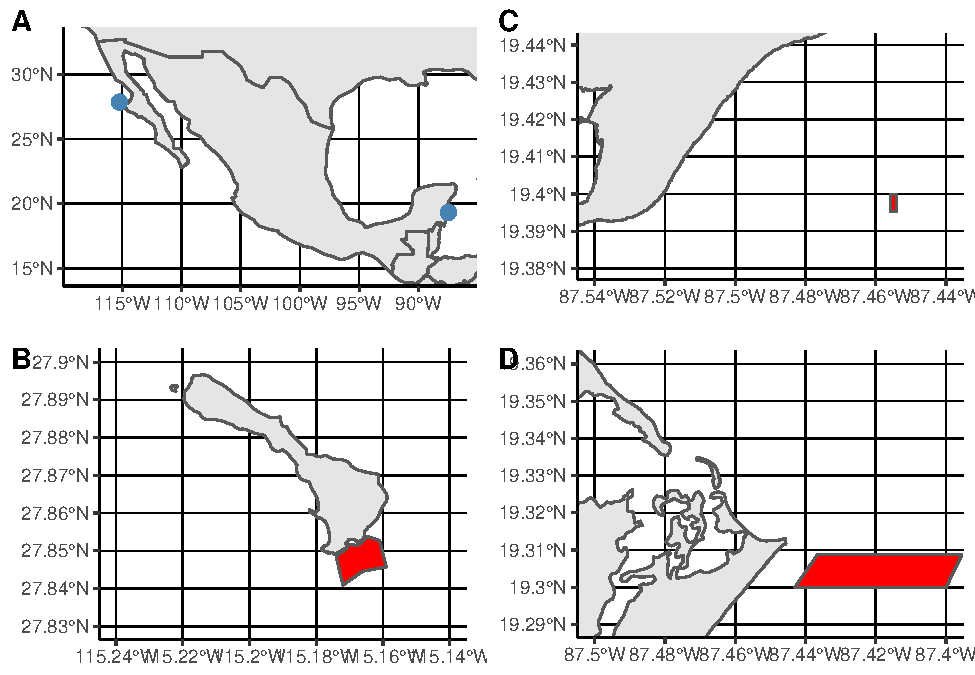
\includegraphics{Villasenor-Derbez_files/figure-latex/unnamed-chunk-1-1.pdf}
\caption{\label{fig:unnamed-chunk-1}\label{fig:map}Location of the three
coastal communities studied (A). Isla Natividad (B) is located off the
Baja California Peninsula, Maria Elena (C) and Punta Herrero (D) are
located in the yucatan Peninsula.}
\end{figure}

\subsection{Data collection}\label{data-collection}

To perform the evaluation of these reserves we use thre sources of
information. Ecological data come from the annual ecological monitorings
of reserve and control areas, carried out by members from each community
and personnel from the Mexican CSO ``Comunidad y Biodiversidad''
(\href{www.cobi.org.mx}{COBI}). These monitorings record richness and
abundances of fish and invertebrate species in the reservs and control
sites. For fish census, size structures are also collected to derive
biomass. We define control sites as regions with habitat characteristics
similar to the corresponding reserves, and that presumably had the same
probability of being selected as reserves during the design phase. From
all the reserves in these three communities, we use the ones that have
data for reserve and control sites before and after the implementation
of the reserve. This provides us with a Before--After--Control--Impact
(\emph{i.e.} BACI) design that allows us to capture and control for
temporal and spatial dynamics \citep{depalma_2018,ferraro_2006-oW}. BACI
designs and causal inference techniques have proven effective to
evaluate marine reserves, as they allow us to causaly attribute observed
changes to the intervention
\citep{moland_2013-VP,Villasenor-Derbez_2018}. All reserves were
surveyed annualy from at least one year before implementation until
2016. Table \ref{tab:com_sum} shows a summary of the number of reserves,
year of implementation, and number of transects for each reserve.

\begin{table}

\caption{\label{tab:unnamed-chunk-2}\label{tab:com_sum} Summary of commuity--based marine reserves by community. Imp = Year of implementation, Start = Year of first sampling, number of fish transects in control (Cf) and reserve (Rf) sites, and number of invertebrate transects in Control (Ci) and Reserve (Ri) sites.}
\centering
\begin{tabular}[t]{l|l|r|r|r|r|r|r}
\hline
Community & Reserve - Control & Imp & Start & Cf & Rf & Ci & Ri\\
\hline
Isla Natividad & La Plana / Las Cuevas - La Dulce / Babencho & 2006 & 2006 & 405 & 242 & 415 & 245\\
\hline
Maria Elena & Cabezo - Cabezo (Control) & 2012 & 2012 & 44 & 45 & 27 & 21\\
\hline
Punta Herrero & El Faro - El Faro (Control) & 2013 & 2013 & 39 & 40 & 24 & 32\\
\hline
Punta Herrero & Manchon - Manchon (Control) & 2013 & 2012 & 43 & 45 & 27 & 42\\
\hline
\end{tabular}
\end{table}

Socioeconomic data come from landing receipts reported to the National
Commission for Aquaculture and Fisheries (\emph{Comisión Nacional de
Acuacultura y Pesca}; CONAPESCA). Data contain monthly lobster landings
(Kg) and value (MXP) from 2000 to 2014. This information was aggregated
by year, and economic values were adjusted by the Consumer Price Index
\citep{oecd_2017-VV} via Eq \ref{eqn:cpi}.

\begin{equation}
I_t = RI_t\times\frac{CPI_t}{CPI_T}
\label{eqn:cpi}
\end{equation}

Where \(I_t\) represents the adjusted income for year \(t\) as the
product between the reported income for that year and the ratio between
the consumer price index in that year (\(CPI_t\)) to the most recent
year's consumer price index (\(CPI_T\)).

\textbf{Governance data were collected at the community--level, using
key informants to collect the necesary information on X, Y, and Z. Algo
mas de Ere.}

\subsection{Data analysis}\label{data-analysis}

Following a framework that relates reserve objectives to performance
indicators \citep{Villasenor-Derbez_2018}, we use five biological, two
socioeconomic, and five governance indicators to evaluate these marine
reserves Table \ref{table:indicators}.

\begin{table}[H]

\caption{\label{tab:unnamed-chunk-3}\label{table:indicators}List of indicators used to evaluate the effectiveness of marine reserves, grouped by category.}
\centering
\begin{tabular}[t]{l|l}
\hline
Category & Indicador\\
\hline
Biological & Abundance\\
\hline
 & Richness\\
\hline
 & Shannon's diversity index\\
\hline
 & Biomass\\
\hline
 & Abundance of target species (lobsters)\\
\hline
Socioeconomic & Income from target species\\
\hline
 & Landings from target species\\
\hline
Governance & Type of access to the fishery\\
\hline
 & Perceived degree of illegal fishing\\
\hline
 & Reserve surveilance anf enforcement\\
\hline
 & Type of fishing organization\\
\hline
 & Age of the reserve\\
\hline
\end{tabular}
\end{table}

Biological indicators are analyzed with a difference--in--differences
analysis (Eq \ref{eqn:reg_bio}), which allows us to estimate the effect
that the reserve has on the biological indicators by comparing trends
across time and treatments
\citep{moland_2013-VP,Villasenor-Derbez_2018}. The analysis is performed
with generalized linear models of the form:

\begin{equation}
I_i = \alpha_{i} + \gamma_{it} Year_t + \beta Zone_i + \lambda_{it} Year_t\times Zone_i + \sigma_jSpp_j + \epsilon
\label{eqn:reg_bio}
\end{equation}

Where year--fixed effects are represented by \(\gamma_{it} Year_t\), and
\(\beta Zone_i\) captures the difference between reserve (\(Zone = 1\))
and control (\(Zone = 0\)) sites. The interaction term
\(\lambda_{it} Year_t\times Zone_i\) represents represent the mean
change in the indicator inside the reserve, for year \(t\), with respect
to the first year of evaluation in the control site (See Table
\ref{tab:com_sum}). When evaluating biomass and abundances, we include
species--fixed effects (\(\sigma_j\)). For abundances and richness
(\emph{i.e.} count data) the model is estimated with a quasipoisson
error distribution.

Socioeconomic indicators are evaluated with a similar approach (Eq
\ref{eqn:soc_reg}), where landings and income before and after the
implementation of the reserve are compared:

\begin{equation}
I_i = \beta_0 + \beta_1Post
\label{eqn:soc_reg}
\end{equation}

This approach does not allow for a causal attribution of the observed
changes to the reserve, but still allows us to draw important
information that can inform our conclusions. For both approaches, model
coefficients are estimated via ordinary least--squares and
heteroskedastic--robust standard errors \citep{zeileis_2004-7n}.

\subsubsection{Governance}\label{governance}

\textbf{Texto de ere y los SES}

\clearpage

\section{Results}\label{results}

Our methodological approach with biological indicators allows us to make
a causal link between the implementation of marine reserves and the
observed trends by accounting for temporal and spatial dynamics
\citep{depalma_2018}. The effect of the reserve is captured by the
\(\lambda_t\) coefficient, and represents the difference observed
between the control site before the implementation of the reserve and
the reserve site at time \(t\) after controling for other time and space
variations (\emph{i.e.} \(\gamma_t\) and \(\beta\) respectively). Here
we present the effect that marine reserves had on each of the biological
indicators for each coastal community, along with the trends in
socioeconomic indicators of lobster catches and revenues. We also
provide an overview of the state of the socioeconomic and governance
settings of each community, and discuss how these dimensions might be
intertwined with each other.

\subsection{Biological}\label{biological}

Effect sizes for biological indicators are shown in Figure
\ref{fig:indicators}. Isla Natividad, the community with the oldest
reserve, shows inconsistent effects across indicators and sources of
data (\emph{i.e.} fish vs.~invertebrates). For example, the reserve had
a small effect on fish abundances (Fig \ref{fig:indicators}A), where
only year 2010 showed significat effect sizes in fish abundances
(\(p<0.05\)) and all other years oscillated above and under zero
(\(p > 0.05\)). However, in the case of invertebrate abundances (Fig
\ref{fig:indicators}B), there was a clear positive effect of the
reserve, as all but 1 year (2008) presented positive effect sizes
relative to the control site (\(p < 0.05\)). Maria Elena and Punta
Herrero showed no significant increase in fish and invertebrate
abundances (\(p< 0.05\)), except for invertebrates in Punta Herrero for
2014 --right after the implementation of the reserves-- which showed a
significant increase (\emph{i.e.} \(\lambda_{2014} = 2.5\),
\(p < 0.05\)). Full tables with model coefficients are presented in the
supplementary materials (\textbf{S1 Table}, \textbf{S2 Table},
\textbf{S3 Table}).

While the number of fish species oscillated above and bellow zero
through time for all reserves, none of these changes were statistically
significant (\(p > 0.05\)) indicating that the reserves had no effect on
fish species richness (Fig \ref{fig:indicators}C). For invertebrate
species in Isla Natividad, all effect sizes were negative, but only
significant for 2008, 2009, 2011, and 2014 (\(p < 0.05\); Fig
\ref{fig:indicators}D). For Maria Elena and Punta Herrero, the data do
not show significant changes in invertebrate species richness
(\(p > 0.05\)).

Effect sizes for Shannon's diversity index for fish (Fig
\ref{fig:indicators}E) in Isla Natividad oscillated between
\(\lambda_{2011} = -0.45\) and \(\lambda_{2010} = -0.005\), but were not
significantly different from null hypotheses of no change (\emph{i.e.}
\(\lambda_t = 0\); \(p > 0.05\)). For invertebrates in that same
community (Fig \ref{fig:indicators}F), Shannon's diversity index showed
a significant decrease between 2008 and 2014, with largest decrease
observed for 2011 (\(\lambda_{2011} = -0.91\); \(p < 0.05\)). In the
case of Maria Elena and Punta Herrero, Shannon's diversity index for
fish showed increases in the order of \(\lambda_t = 1\). For Maria Elena
and Punta Herrero, these effects were only statistically significant for
2014, and 2014 and 2015 (\(p < 0.05\)).

Biomass was only evaluated for fish data (Fig \ref{fig:indicators}G). In
Isla Natividad, fish biomass presented a steady but small increase
(\(p>0.05\)), and exhibited an increased variability in biomass between
2013 and 2016. Maria Elena and Punta Herrero also showed small,
non-statistically significant increases in fish biomass (\(p>0.05\)).
The last biological indicator is abundance of target species,
\emph{Panulirus interruptus} and \emph{P. argus}, for the Pacific and
Caribbean, respectively (Fig \ref{fig:indicators}H). Isla Natividad
presented small constantly-positive effects but were not significantly
different from the reference point of control site before the
implementation of the reserve (\(p > 0.05\). Maria Elena showed
significant increases in lobster densities in the order of
\(\lambda_t = 10\) (\(p < 0.05\)). Finally, punta herrero presented
alternating negative and positive effects, but these were not different
from the baseline case (\(p > 0.05\)).

\begin{figure}
\centering
\includegraphics{Villasenor-Derbez_files/figure-latex/unnamed-chunk-4-1.pdf}
\caption{\label{fig:unnamed-chunk-4}\label{fig:indicators}Effect sizes for
marine reserves from Isla Natividad (IN; red cirlcles), Maria Elena (ME;
blue triangles), and Punta Herrero (PH; green squares) for
community-levell indicators. Plots are ordered by survey type (left:
fish; right: invertebrates) and indicators: Abundance (A, B), Richness
(C, D), Shannon's diversity index (E, F),fish biomass (G), and lobster
(\emph{Panulirus spp}) abundances (H). Points are jittered hotizontally
to avoid overplotting. Points indicate the effect size, and errorbars
are heteroskedastic-robust standard errors.}
\end{figure}

\subsection{Socioeconomic}\label{socioeconomic}

\begin{figure}
\centering
\includegraphics{Villasenor-Derbez_files/figure-latex/unnamed-chunk-5-1.pdf}
\caption{\label{fig:unnamed-chunk-5}\label{fig:lobsters}Time series of
lobster catches (A) and revenues (B) in at Isla Natividad (IN; red
circles), Maria Elena (ME; blue triangles), and Punta Herrero (PH; green
squares).}
\end{figure}

\subsection{Governance}\label{governance-1}

\section{Discussion}\label{discussion}

The biological effects of the reserve contrast the existing literature.
Why no effect on bio? IN hypoxia. ME and PH, age? Perhaps is the use of
causal inference methods?

Isla natividad no funciona por hipoxya

Maria Elena funciona ``bien''

Punta Herrero no funciona por poaching.

Aun con las mejores caracteristicas sociales, noe s posible vencer al
ambiente (IN). Para el Caribe, parece ser que buena vigilancia y poca
pesca ilegal son determinantes para obtener buenos resultados.
Preguntarle a Stuart si ME solamente se pesca durante lanosta, y todo el
ano es reserva.

IN captures more dynamics. Reflects hypoxia events. Citar paper Giron

Differences between fish and inverts sheds a lights on direct and
indirect effects (Paper que recomendo Fio).

\section*{Conflict of Interest Statement}

The authors declare that the research was conducted in the absence of
any commercial or financial relationships that could be construed as a
potential conflict of interest.

\section*{Author Contributions}

JC and EA analyzed and interpreted data, discussed the results and wrote
the manuscrip. SF and JT edited the manuscript and discussed the
results.

\section*{Funding}

Details of all funding sources should be provided, including grant
numbers if applicable. Please ensure to add all necessary funding
information, as after publication this is no longer possible.

\section*{Acknowledgments}

This is a short text to acknowledge the contributions of specific
colleagues, institutions, or agencies that aided the efforts of the
authors.

\section*{Supplemental Data}

\href{http://home.frontiersin.org/about/author-guidelines#SupplementaryMaterial}{Supplementary Material}
should be uploaded separately on submission, if there are Supplementary
Figures, please include the caption in the same file as the figure.
LaTeX Supplementary Material templates can be found in the Frontiers
LaTeX folder

\paragraph*{S1 Figure}
\label{S1_Figure}

Timeseries of indicators for IN

\paragraph*{S2 Figure}
\label{S2_Figure}

Timeseries of indicators for ME

\paragraph*{S3 Figure}
\label{S3_Figure}

Timeseries of indicators for PH

\paragraph*{S1 Table}
\label{S1_Table}

Coefficient estimates for Isla Natividad

\paragraph*{S2 Table}
\label{S2_Table}

Coefficient estimates for Maria Elena

\paragraph*{S3 Table}
\label{S3_Table}

Coefficient estimates for Punta Herrero

\bibliographystyle{frontiersinSCNS_ENG_HUMS}\bibliography{references}

\section*{Figure captions}



\end{document}
